
\begin{frame}\frametitle{Allowed decay modes}
\centering\myskip

\begin{minipage}{.4\textwidth}\centering
\scriptsize
  \begin{tabular}{cc}\toprule
Singlet & Decay modes\\ 
& \\
$T(+2/3)$ & ${\cccolor W^+b},\, {\cccolor Ht},\, Zt$ \\
& \\
$B(-1/3)$ & $ W^-t,\, Hb,\, Zb$ \\
& \\
$X(+5/3)$ & $W^+t$\\
& \\
$Y(-4/3)$ & \cccolor$W^-b$ \\
& \\\midrule
Doublet & Decay modes\\
 &\\
 \multirow{2}{*}{$\bigg(\begin{array}{c}T \\ B\end{array}\bigg)$} & ${\cccolor W^+b},\, {\cccolor Ht},\, Zt$ \\
 & $ W^-t,\, Hb,\, Zb$\\
 & \\
\multirow{2}{*}{$\bigg(\begin{array}{c}T \\ X\end{array}\bigg)$} & ${\cccolor Ht},\, Zt$\\
 & $W^+t$\\
 &\\
 \multirow{2}{*}{$\bigg(\begin{array}{c}B \\ Y\end{array}\bigg)$} & $Hb,\, Zb$\\
 & \cccolor$W^-b$\\
\bottomrule
\end{tabular}

\end{minipage}\begin{minipage}{.6\textwidth}\centering
  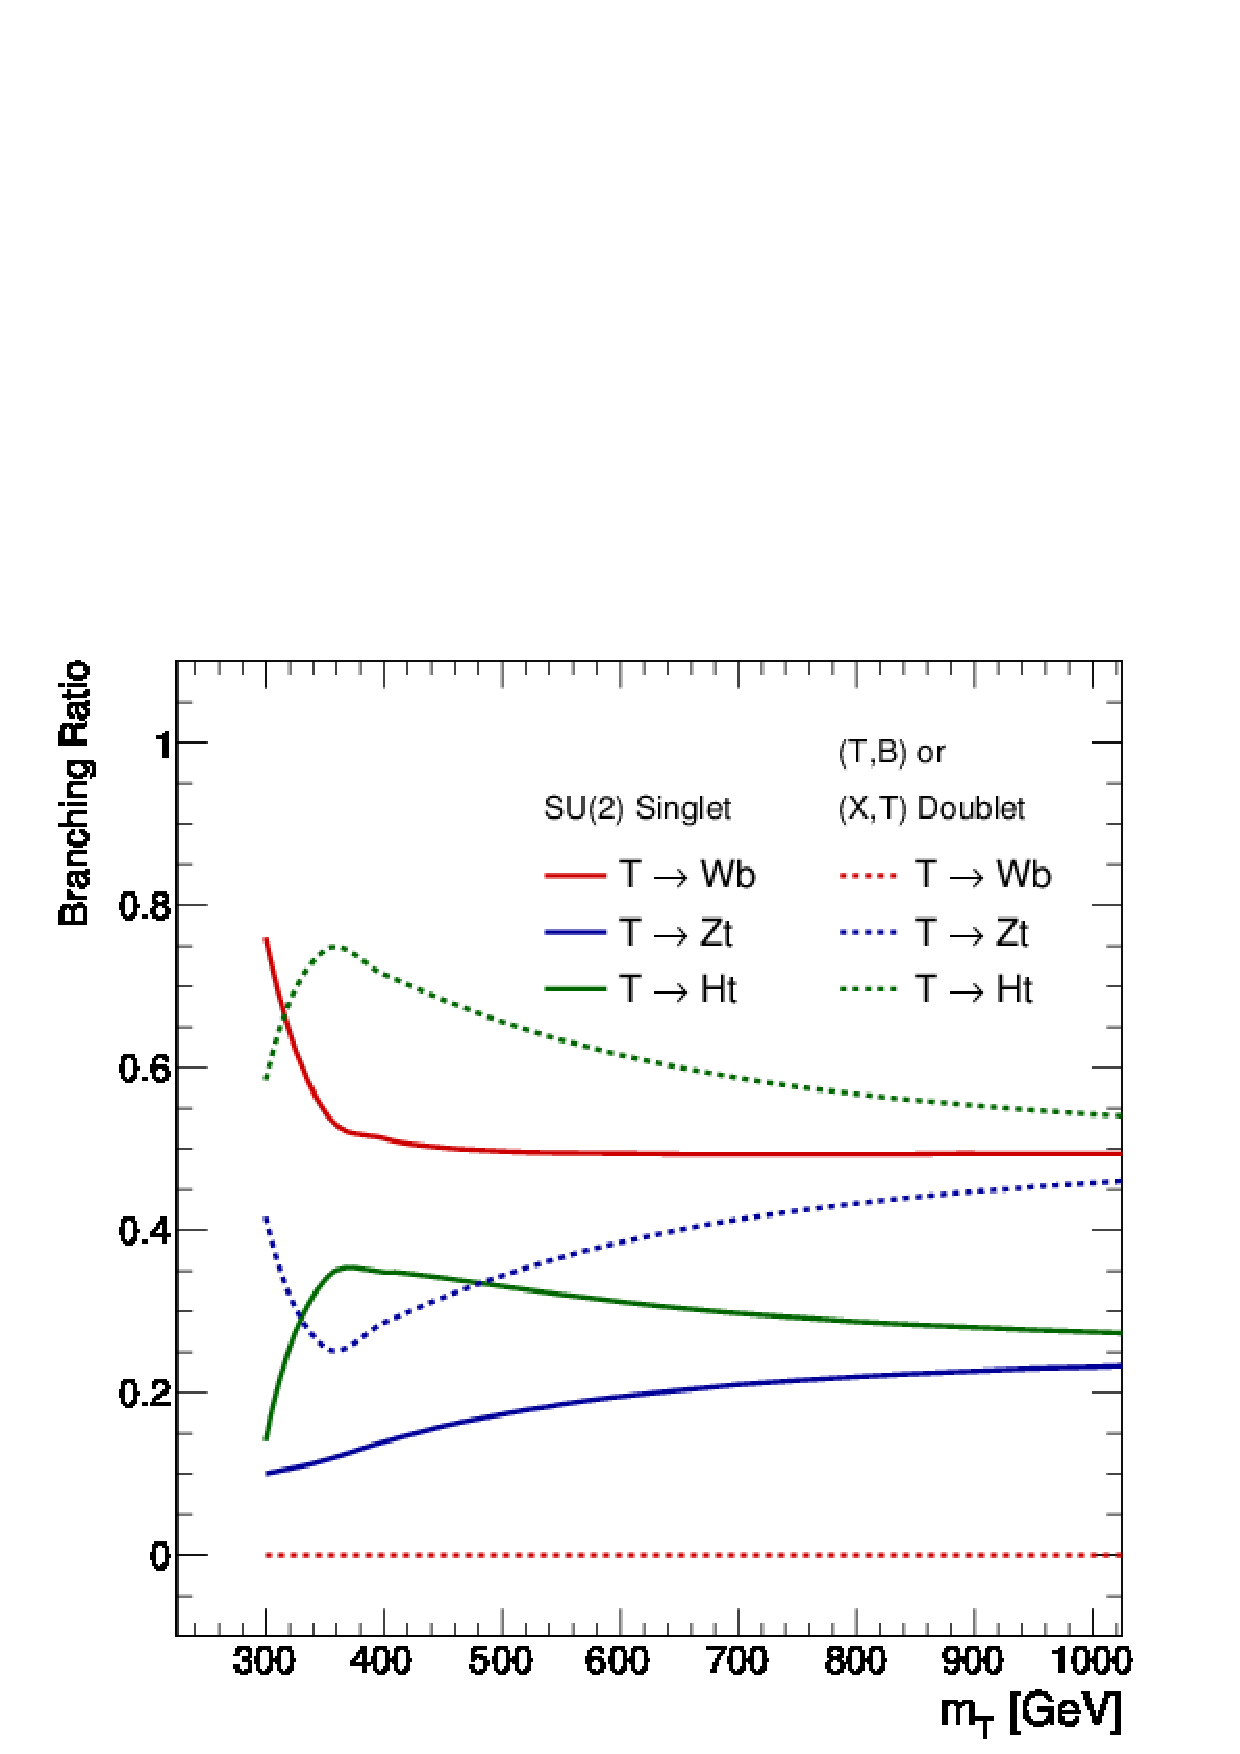
\includegraphics[width=0.95\textwidth]{../vlq_analysis/figures/fig_02a.pdf}
\end{minipage}

\end{frame}




\begin{frame}\frametitle{Model Independent Strategy}
\footnotesize\centering


\begin{pgfpicture}{0.0\textwidth}{0.0\textheight}{1.\textwidth}{.6\textwidth}

\begin{pgfscope}
\pgfdeclareimage[interpolate=true,width=.45\textwidth]{tab}{pics/tabBRs}
\onslide<1->{
    \pgfsetendarrow{\pgfarrowlargepointed{6pt}}
    \pgfsetlinewidth{1.5pt}
    \usebeamercolor[fg]{head/foot boxes}
    \begin{pgftranslate}{\pgfpoint{0.07\textwidth}{0.15\textheight}}
\pgfline{\pgfxy(0,0)}{\pgfxy(5.5,0)}
\pgfstroke
\pgfputat{\pgfxy(3.5,-0.5)}{\pgfbox[left,base]{BR($T\to Wb$)}}
    \usebeamercolor[fg]{normal text}
\pgfcircle[fill]{\pgfxy(6.8,4.1)}{2pt}
\pgfputat{\pgfxy(7,4)}{\pgfbox[left,base]{Build a 2-dim plane}}
\pgfputat{\pgfxy(7,3.7)}{\pgfbox[left,base]{to scan model mixing}}
%    \end{pgftranslate}
%\end{pgfscope}
}
%\pause
\onslide<2->{
%\begin{pgfscope}
    \pgfsetendarrow{\pgfarrowlargepointed{6pt}}
    \pgfsetlinewidth{1.5pt}
    \usebeamercolor[fg]{head/foot boxes}
%    \begin{pgftranslate}{\pgfpoint{0.1\textwidth}{0.15\textheight}}
    \usebeamercolor[fg]{head/foot boxes}
\pgfline{\pgfxy(0,0)}{\pgfxy(0,5.5)}
\pgfstroke
    \begin{pgfrotateby}{\pgfdegree{90}}
\pgfputat{\pgfxy(3.5,0.4)}{\pgfbox[left,base]{BR($T\to Ht$)}}
    \end{pgfrotateby}
%    \end{pgftranslate}
%\end{pgfscope}
    \usebeamercolor[bg]{head/foot boxes}
    \pgfcircle[fill]{\pgfxy(5.,0)}{3pt}
    \pgfcircle[fill]{\pgfxy(2.5,1.5)}{3pt}
    \pgfcircle[fill]{\pgfxy(0.,3.)}{3pt}
    \pgfputat{\pgfxy(5.5,4.7)}{\pgfbox[left,base]{\pgfuseimage{tab}}}
}
%\pause
\onslide<3->{
%\begin{pgfscope}
    \pgfsetlinewidth{1.5pt}
    \color{light-gray}
%    \begin{pgftranslate}{\pgfpoint{0.1\textwidth}{0.15\textheight}}
%\pgfline{\pgfxy(5,0)}{\pgfxy(0,5)}
%\pgfstroke
\pgfmoveto{\pgfxy(5,0)}
\pgflineto{\pgfxy(5,5)}
\pgflineto{\pgfxy(0,5)}
%\pgfstroke
\pgffill
    \color{gray}
\pgfputlabelrotated{0.5}{\pgfxy(0,5)}{\pgfxy(5,0)}{8pt}{\pgfbox[center,base]{Forbidden}}
    \usebeamercolor[fg]{normal text}
\pgfcircle[fill]{\pgfxy(6.8,3.3)}{2pt}
\pgfputat{\pgfxy(7,3.2)}{\pgfbox[left,base]{Sum of BRs is 1$^{(a)}$}}
%\pgfputat{\pgfxy(5.2,0.7)}{\pgfbox[left,base]{\scriptsize $^{(a)}$BR($T\to  Zt/b$) = 1 - BR($T\to Ht/b$) - BR($T\to Wb/t$)}}
\pgfputat{\pgfxy(5.9,-0.9)}{\pgfbox[left,base]{\scriptsize $^{(a)}$BR($T\to  Zt$) = 1 - BR($T\to Ht$) - BR($T\to Wb$)}}
%\pgfputat{\pgfxy(8.755,-0.7)}{\pgfbox[left,base]{\scriptsize - BR($T\to Wb$)}}
{
    \usebeamercolor[bg]{head/foot boxes}
    \pgfcircle[fill]{\pgfxy(5.,0)}{3pt}
}
%    \end{pgftranslate}
%\end{pgfscope}
}
%\pause
\onslide<4->{
%\begin{pgfscope}
    \pgfsetlinewidth{1.5pt}
%    \begin{pgftranslate}{\pgfpoint{0.1\textwidth}{0.15\textheight}}
    \usebeamercolor[fg]{normal text}
\pgfcircle[fill]{\pgfxy(6.8,2.8)}{2pt}
\pgfputat{\pgfxy(7,2.7)}{\pgfbox[left,base]{Different analyses are}}
\pgfputat{\pgfxy(7,2.4)}{\pgfbox[left,base]{sensitive to different areas}}
    \usebeamercolor[fg]{head/foot boxes}
\begin{pgfscope}
\pgfmoveto{\pgfxy(5,0)}
\pgflineto{\pgfxy(0,0)}
\pgflineto{\pgfxy(0,5)}
\pgfclip
\pgfcircle[fill]{\pgfxy(.5,4)}{55pt}
{\usebeamercolor[bg]{normal text}
%\pgfputat{\pgfxy(0.,3.5)}{\begin{pgfrotateby}{\pgfdegree{-45}}\pgfbox[left,base]{$T(B)\to Ht(b)$}\end{pgfrotateby}}
\pgfputat{\pgfxy(0.05,3.2)}{\pgfbox[left,base]{\large$Ht+X$}}
}
{
    \usebeamercolor[bg]{head/foot boxes}
    \pgfcircle[fill]{\pgfxy(0.,3.)}{3pt}
}
}
\pgfcircle[fill]{\pgfxy(4,0)}{35pt}
{\usebeamercolor[bg]{normal text}
%\pgfputat{\pgfxy(3.,0.4)}{\pgfbox[left,base]{$T(B)\to Wb(t)$}}
\pgfputat{\pgfxy(2.9,0.2)}{\pgfbox[left,base]{\large$Wb+X$}}
}
{
    \usebeamercolor[bg]{head/foot boxes}
    \pgfcircle[fill]{\pgfxy(5.,0)}{3pt}
}
\end{pgfscope}
\onslide<5->{
\usebeamercolor[fg]{normal text}
%\pgfcircle[fill]{\pgfxy(6.8,2.)}{2pt}
%\pgfputat{\pgfxy(7,1.9)}{\pgfbox[left,base]{Set exclusion using $CL_{s}$ }}
%\pgfputat{\pgfxy(7,1.6)}{\pgfbox[left,base]{in each point of the plane}}
%\pgfcircle[fill]{\pgfxy(6.8,1.2)}{2pt}
\pgfputat{\pgfxy(5.3,1.)}{\pgfbox[left,base]{\begin{tabular}{c c c} 
Set strategy & \multirow{2}{*}{$\Rightarrow$} & Check good bkg \\
($S/B$)      &                                & modeling \\
             &                                &  $\Downarrow$\\
Test \cls{b} and & \multirow{2}{*}{$\Leftarrow$} & \multirow{2}{*}{Look at data} \\
\cls{s+b} hypotheses & &\\
\multicolumn{3}{c}{$\nwarrow$} \\
\multicolumn{3}{c}{\it for each point of the BR plane}\\
\end{tabular}}}
}
    \end{pgftranslate}
\end{pgfscope}
\end{pgfpicture}

\end{frame}





\begin{frame}\frametitle{Preselection}
\centering\myskip

\begin{minipage}{.6\textwidth}\centering\footnotesize
Two searches using common analysis framework:
\begin{minipage}{.5\textwidth}\centering
\begin{itemize}
\item \wbx
\end{itemize}
\scriptsize
\cccolor 

ATLAS-CONF-2013-060~\cite{ATLAS-CONF-2013-060}
\end{minipage}\begin{minipage}{.5\textwidth}\centering
\begin{itemize}
\item \htx
\end{itemize}
\scriptsize
\cccolor 

ATLAS-CONF-2013-018~\cite{ATLAS-CONF-2013-018}
\end{minipage}

\myskip

\begin{tabular}{ll}
\toprule
Preselection stage & Requirements \\
\midrule
Single lepton & One electron or muon\\
              & matching trigger  \\\midrule
%\\
QCD rejection & $\met >20\gev$\\
              & $\met +m_{\rm T}>60\gev$ \\\midrule
%\\
Jet multiplicity & $\geq 4$ jets\\
                 & $\geq 1$ $b$-tagged jets \\
\bottomrule\end{tabular}

\myskip
{\bfseries\cccolor + ``orthogonality'' requirements} 

\myskip

\end{minipage}\begin{minipage}{.4\textwidth}\centering
\vskip-5ex
\includegraphics[width=0.9\textwidth]{pics/feyn_wbwb}\\
\vskip-2ex
\includegraphics[width=0.9\textwidth]{pics/feyn_htX}
\end{minipage}


\end{frame}



\begin{frame}\frametitle{Background and signal modelling}
\centering\myskip

\begin{minipage}{.5\textwidth}\footnotesize\centering
\scriptsize
Yields in the preselection region ``blinded'' as:\\
$\htfj<800\gev$ (*)
\myskip

  \input{tabs/blinded_presel}

\myskip
(*) $\htfj = \pT(l) + \met + \sum_{j = 1}^{\rm 4}\pT(j)$

\begin{pgfpicture}{0.0\textwidth}{0.0\textheight}{1.\textwidth}{.01\textwidth}
\pgfdeclareimage[interpolate=true,width=0.8\textwidth]{ttalp}{pics/Njets25_ELEMUON_4jetin1btagin_NOMINAL}
\begin{pgfscope}
 \pgfsetlinewidth{1.pt}
 \usebeamercolor[bg]{head/foot boxes}
 \pgfrect[stroke]{\pgfxy(0,4.15)}{\pgfxy(6,0.35)}
\only<2>{
\pgfputat{\pgfxy(0.8,0.2)}{\pgfbox[left,base]{\pgfuseimage{ttalp}}}
}
\end{pgfscope}
\end{pgfpicture}

\end{minipage}\begin{minipage}{.5\textwidth}\footnotesize\centering

\only<1>{
\begin{itemize}
\item $t\bar{t}$ pair production in association with jets generated with {\tt MC@NLO}+{\tt HERWIG}
\item $m_t = 172.5\gev$
\item NNLO theoretical cross section
\end{itemize}

but\\
{\tt MC@NLO} does not model well high-jet multiplicity regions!

}

\only<2>{
\begin{itemize}
\item Additional samples generated with {\tt ALPGEN}+{\tt HERWIG}
\item Separate samples are generated for $t\bar{t}$+light jets with up to three additional light partons,
and for $t\bar{t}$+heavy-flavour jets including $t\bar{t}b\bar{b}$ and $t\bar{t}c\bar{c}$ 
\item $m_t = 172.5\gev$
\item NNLO theoretical cross section
\end{itemize}

Yields for \ttbar\ predicted with \texttt{ALPGEN}
are $\sim$3-8\% higher than \texttt{MC@NLO}

%\includegraphics[width=0.8\textwidth]{pics/Njets25_ELEMUON_4jetin1btagin_NOMINAL}

}

\end{minipage}

\end{frame}


\begin{frame}\frametitle{Background and signal modelling}
\centering\myskip

\begin{minipage}{.5\textwidth}\footnotesize\centering
\scriptsize
Yields in the preselection region ``blinded'' as:\\
$\htfj<800\gev$ (*)
\myskip

  \input{tabs/blinded_presel}

\myskip
(*) $\htfj = \pT(l) + \met + \sum_{j = 1}^{\rm 4}\pT(j)$

\begin{pgfpicture}{0.0\textwidth}{0.0\textheight}{1.\textwidth}{.01\textwidth}
\begin{pgfscope}
 \pgfsetlinewidth{1.pt}
 \usebeamercolor[bg]{head/foot boxes}
 \pgfrect[stroke]{\pgfxy(0,3.5)}{\pgfxy(6,0.7)}
\end{pgfscope}
\end{pgfpicture}

\end{minipage}\begin{minipage}{.5\textwidth}\footnotesize\centering


\begin{itemize}
\item $W$ and $Z$ boson production in association with jets generated with up to five additional partons with {\tt ALPGEN}+{\tt HERWIG}
\end{itemize}

$W$+jets:
\begin{itemize}
\item Samples generated separately for $W$+light jets, $Wb\bar{b}$+jets, $Wc\bar{c}$+jets, and $Wc$+jets
\item Normalized to data-driven prediction
\end{itemize}

$Z$+jets:
\begin{itemize}
\item Samples generated separately for $Z$+light jets, $Zb\bar{b}$+jets, and $Zc\bar{c}$+jets 
\item Inclusive NNLO theoretical cross section
\end{itemize}

\end{minipage}
\end{frame}




\begin{frame}\frametitle{Background and signal modelling}
\centering\myskip

\begin{minipage}{.5\textwidth}\centering
\scriptsize
Yields in the preselection region ``blinded'' as:\\
$\htfj<800\gev$ (*)
\myskip

  \input{tabs/blinded_presel}

\myskip
(*) $\htfj = \pT(l) + \met + \sum_{j = 1}^{\rm 4}\pT(j)$


\begin{pgfpicture}{0.0\textwidth}{0.0\textheight}{1.\textwidth}{.01\textwidth}
\begin{pgfscope}
 \pgfsetlinewidth{1.pt}
 \usebeamercolor[bg]{head/foot boxes}
 \pgfrect[stroke]{\pgfxy(0,3.27)}{\pgfxy(6,0.35)}
\end{pgfscope}
\end{pgfpicture}

\end{minipage}\begin{minipage}{.5\textwidth}\footnotesize
\centering

\begin{itemize}
\item QCD multi-jet events have high cross-section
\item Jets are misidentified as leptons
\item Data-driven estimation (Matrix-method)
\end{itemize}

\includegraphics[width=0.4\textwidth]{../vlq_analysis/figures/mm_regions}

\myskip

\begin{minipage}{.7\textwidth}\footnotesize
$N^\mathrm{loose}  =  N^\mathrm{loose}_\mathrm{real} + N^{loose}_\mathrm{fake}$ \\\myskip
$N^\mathrm{tight}  =  \epsilon_\mathrm{real}N^\mathrm{loose}_\mathrm{real} + \epsilon_\mathrm{fake}N^\mathrm{loose}_\mathrm{fake}$
\end{minipage}

%N^\mathrm{tight}_\mathrm{fake} = \frac{\epsilon_\mathrm{fake}}{\epsilon_\mathrm{real} - \epsilon_\mathrm{fake}}(N^\mathrm{loose} \epsilon_\mathrm{real} - N^\mathrm{tight})$$

\end{minipage}
\end{frame}


\begin{frame}\frametitle{Background and signal modelling}
\centering\myskip

\begin{minipage}{.5\textwidth}\footnotesize\centering
\scriptsize
Yields in the preselection region ``blinded'' as:\\
$\htfj<800\gev$ (*)
\myskip

  \input{tabs/blinded_presel}

\myskip
(*) $\htfj = \pT(l) + \met + \sum_{j = 1}^{\rm 4}\pT(j)$

\begin{pgfpicture}{0.0\textwidth}{0.0\textheight}{1.\textwidth}{.01\textwidth}
\begin{pgfscope}
 \pgfsetlinewidth{1.pt}
 \usebeamercolor[bg]{head/foot boxes}
 \pgfrect[stroke]{\pgfxy(0,2.7)}{\pgfxy(6,0.6)}
\end{pgfscope}
\end{pgfpicture}

\end{minipage}\begin{minipage}{.5\textwidth}\footnotesize\centering

Single top:
\begin{itemize}
\item $s$-channel and $Wt$ production generated with {\tt MC@NLO}+{\tt HERWIG}
\item $t$-channel generated with {\tt ACERMC}+{\tt PYTHIA}
\item $m_t = 172.5\gev$
\item NNLO theoretical cross sections
\end{itemize}

Diboson:

\begin{itemize}
\item Diboson production generated with {\tt HERWIG}
\item NLO theoretical cross section
\end{itemize}

\end{minipage}
\end{frame}



\begin{frame}\frametitle{Background and signal modelling}
\centering\myskip

\begin{minipage}{.5\textwidth}\footnotesize\centering
\scriptsize
Yields in the preselection region ``blinded'' as:\\
$\htfj<800\gev$ (*)
\myskip

  \input{tabs/blinded_presel}

\myskip
(*) $\htfj = \pT(l) + \met + \sum_{j = 1}^{\rm 4}\pT(j)$

\begin{pgfpicture}{0.0\textwidth}{0.0\textheight}{1.\textwidth}{.01\textwidth}
\begin{pgfscope}
 \pgfsetlinewidth{1.pt}
 \usebeamercolor[bg]{head/foot boxes}
 \pgfrect[stroke]{\pgfxy(0,2.15)}{\pgfxy(6,0.6)}
\end{pgfscope}
\end{pgfpicture}

\end{minipage}\begin{minipage}{.5\textwidth}\footnotesize\centering

$t\bar{t}V$:
\begin{itemize}
\item $t\bar{t}$ produced in association with a $W$ or $Z$ boson generated with {\tt MADGRAPH}+{\tt PYTHIA}
\item $m_t = 172.5\gev$
\item NLO theoretical cross section
\end{itemize}

$t\bar{t}H$:
\begin{itemize}
\item $t\bar{t}$ produced in association with a Higgs boson generated with {\tt PYTHIA}
\item $m_t = 172.5\gev$, $m_H=125\gev$
\item Higgs decay modes considered: $H\to b\bar{b}$, $c\bar{c}$, $gg$, $W^+W^-$
\item NLO theoretical cross section
\end{itemize}

\end{minipage}
\end{frame}



\begin{frame}\frametitle{Background and signal modelling}
\centering\myskip

\begin{minipage}{.5\textwidth}\footnotesize\centering
\scriptsize
Yields in the preselection region ``blinded'' as:\\
$\htfj<800\gev$ (*)
\myskip

  \input{tabs/blinded_presel}

\myskip
(*) $\htfj = \pT(l) + \met + \sum_{j = 1}^{\rm 4}\pT(j)$

\begin{pgfpicture}{0.0\textwidth}{0.0\textheight}{1.\textwidth}{.01\textwidth}
\begin{pgfscope}
 \pgfsetlinewidth{1.pt}
 \usebeamercolor[bg]{head/foot boxes}
 \pgfrect[stroke]{\pgfxy(0,1.2)}{\pgfxy(6,0.35)}
\end{pgfscope}
\end{pgfpicture}

\end{minipage}\begin{minipage}{.5\textwidth}\footnotesize\centering

\begin{itemize}
\item \TTbar\ singlet production generated with {\tt PROTOS}+{\tt PYTHIA}
\item Branching ratio to each decay mode  ($Wb$, $Zt$ and $Ht$) is set to  1/3
\item Events are reweighted at the analysis level in order to reproduce any desired branching ratio configuration
\item $m_{T}$ values generated from $350\gev$ to $850\gev$ in steps of $50\gev$
\item $m_H=125\gev$, all Higgs boson decay modes are considered
\item NNLO theoretical cross section
\end{itemize}

\end{minipage}


\end{frame}

\begin{frame}\frametitle{Systematic uncertainties - Shape and Norm}
\centering\myskip\scriptsize

\resizebox{!}{.28\textwidth}{
\begin{tabular}{lcccc}
\toprule
Systematic uncertainty & \multicolumn{2}{c}{ \wbx\  } & \multicolumn{2}{c}{ \htx\  }\\
 & Status  & Components & Status  & Components\\
\midrule
Luminosity                  &  N & 1 &  N & 1\\
Lepton ID+reco+trigger      &  N & 1 &  N & 1\\
\rowcolor{TabLight}Jet energy scale            & SN & 1 & SN & 8\\
Jet energy resolution       & SN & 1 & SN & 1\\
%Jet mass scale               & - & -\\
%Jet mass resolution      & - & -\\
Jet vertex fraction efficiency & SN & 1 & SN & 1\\
\rowcolor{TabLight}$b$-tagging efficiency      & SN & 9 & SN & 9\\
$c$-tagging efficiency      & SN & 5 & SN & 5\\
Light jet-tagging efficiency    & SN & 1 & SN & 1\\\midrule
$t\bar{t}$ cross section    &  N & 1 &  N & 1\\
$t\bar{t}V$ cross section   &  N & 1 &  N & 1\\
$t\bar{t}H$ cross section   & - & - &  N & 1\\
Dibosons cross section      &  N & 1 &  N & 1\\
Single top cross section    &  N & 1 &  N & 1\\\midrule
$W$+jets normalization      &  N & 5 &  - & -\\
$Z$+jets normalization      &  N & 1 &  - & -\\
$V$+jets normalization      &  - & - &  N & 1\\
Multijet normalization      &  - & - &  N & 1\\
\rowcolor{TabLight}$t\bar{t}$ modelling        & SN & 3 & SN & 3\\
$V$+jets modelling         & SN & 1 &  - & -\\
$t\bar{t}$+heavy-flavour fractions &  - & -& N & 1\\
%$\TT$ modelling        & - & -\\
\bottomrule
\end{tabular}
}

\end{frame}

